\documentclass[12pt]{article}

\usepackage[a4paper, total={6in, 9in}]{geometry}
\usepackage[hidelinks]{hyperref}
\hypersetup{
    colorlinks=true,
    linkcolor=blue,    
    urlcolor=cyan,
    pdfborder={0 0 0},       % Disables the border around links
    linkbordercolor={0 0 0}, % Disables yellow hover highlighting
}
\usepackage[english, activeacute]{babel}
\usepackage[utf8]{inputenc}
\usepackage[T1]{fontenc}
\usepackage{amsmath}
\usepackage{graphicx}
\usepackage{float}
\usepackage{amsthm}
\usepackage{amsfonts}
\usepackage{bookmark}
\usepackage{enumitem}
\usepackage[parfill]{parskip}
\usepackage{minted} 
\usepackage{multicol}
\usepackage{caption}
\usepackage{graphicx} % Package to insert images
\graphicspath{ {images/} } % Path to images directory

\title{Preliminary Report}
\author{Diego Chiola, Alex Valle, Gabriele Berruti}
\date{10/01/2025}

\begin{document}
\maketitle
\newpage

\section{Topic}
The main topic of our final project will be about digitalization in the European
Union countries, more precisely we want to analyze three aspects:
\begin{enumerate}
    \item \textbf{The level of access to the internet}: how many have access to the
          internet, with which devices and how this percentage has changed over time
    \item \textbf{Internet uses}: how often people use the internet, for what purposes,
          negative experiences of users, to then do a more in-depth analysis for some
          sectors such as e-commerce and financial activities.
    \item \textbf{Digital skills}: the skills that people have in using the internet,
          the skills in evaluating the information they find online and the number
          of people who have ICT skills.
\end{enumerate}

\section{Datasets}
Digitalization
\href{https://ec.europa.eu/eurostat/web/digital-economy-and-society/database}{datasets}
\begin{itemize}
    \item Internet access section:
          \begin{itemize}
              \item Households - level of internet access
              \item Households - type of connection to the internet
              \item Households - devices to access the internet
              \item Households - reasons for not having internet access at home
          \end{itemize}

    \item Frequency and use type of internet:
          \begin{itemize}
              \item Individuals - frequency of internet use
              \item Individuals - internet activities
              \item Individuals - encountering hostile or degrading online messages
              \item Internet purchases by individuals
              \item Financial activities over the internet
          \end{itemize}
    \item Digital skill
          \begin{itemize}
              \item Individuals' level of digital skills
              \item Evaluating data, information and digital content
              \item Persons with ICT education by labour status
              \item ICT specialist in employment (by sex, age and educational attainment level)
          \end{itemize}
\end{itemize}
\section{Charts type}
\subsection*{Bar chart}
\begin{figure}[h]
    \centering
    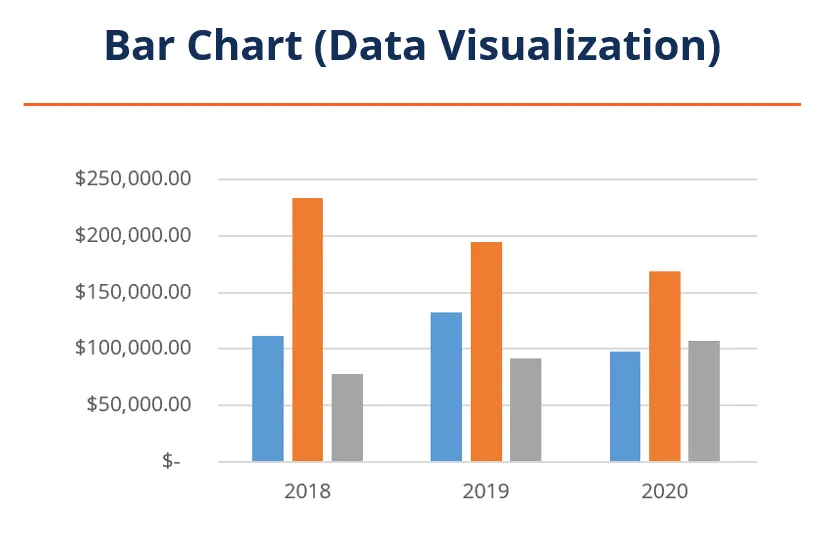
\includegraphics[width=10cm, height=7cm]{bar-charts.png}
    \centering
\end{figure}

\subsection*{Stacked Bar Chart}
\begin{figure}[h]
    \centering
    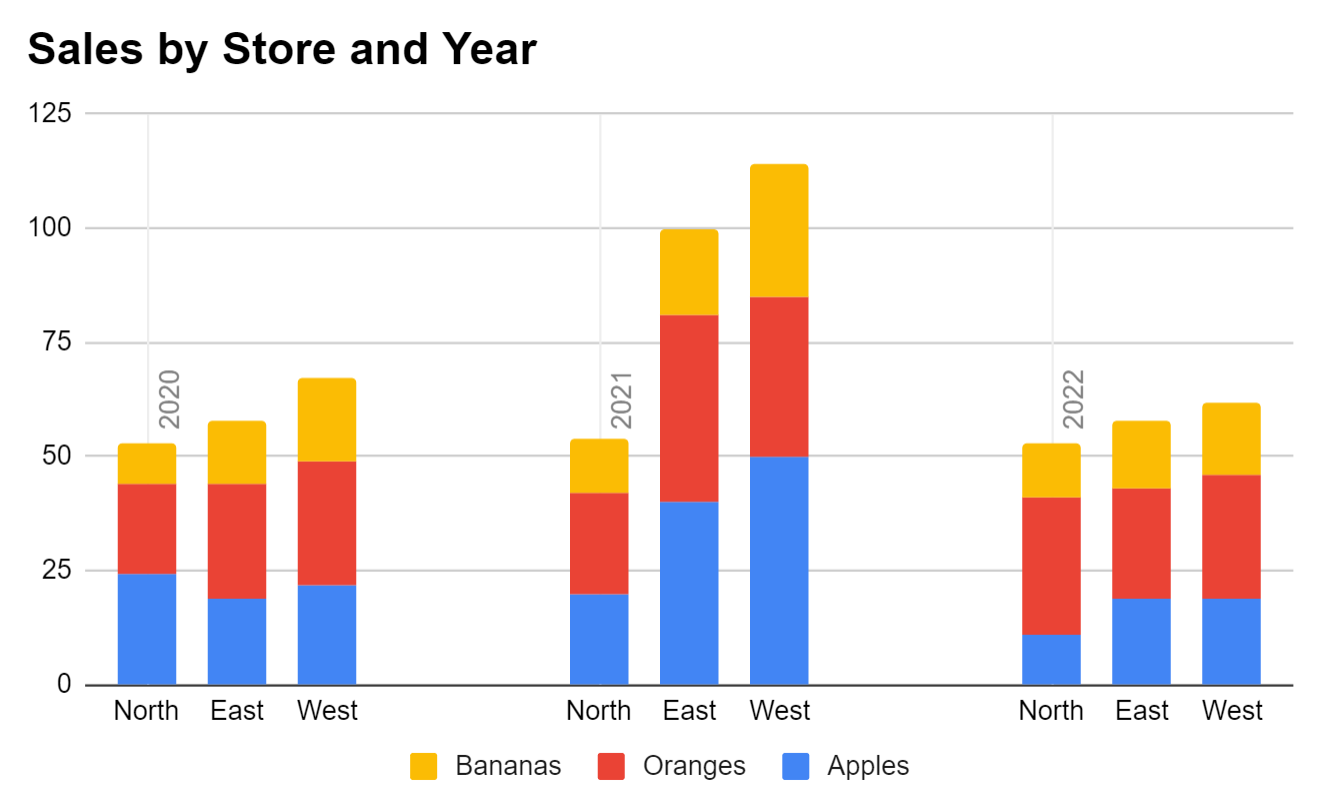
\includegraphics[width=10cm, height=7cm]{clusterstack1.png}
    \centering
\end{figure}

\newpage

\subsection*{Alluvial Chart}
\begin{figure}[h]
    \centering
    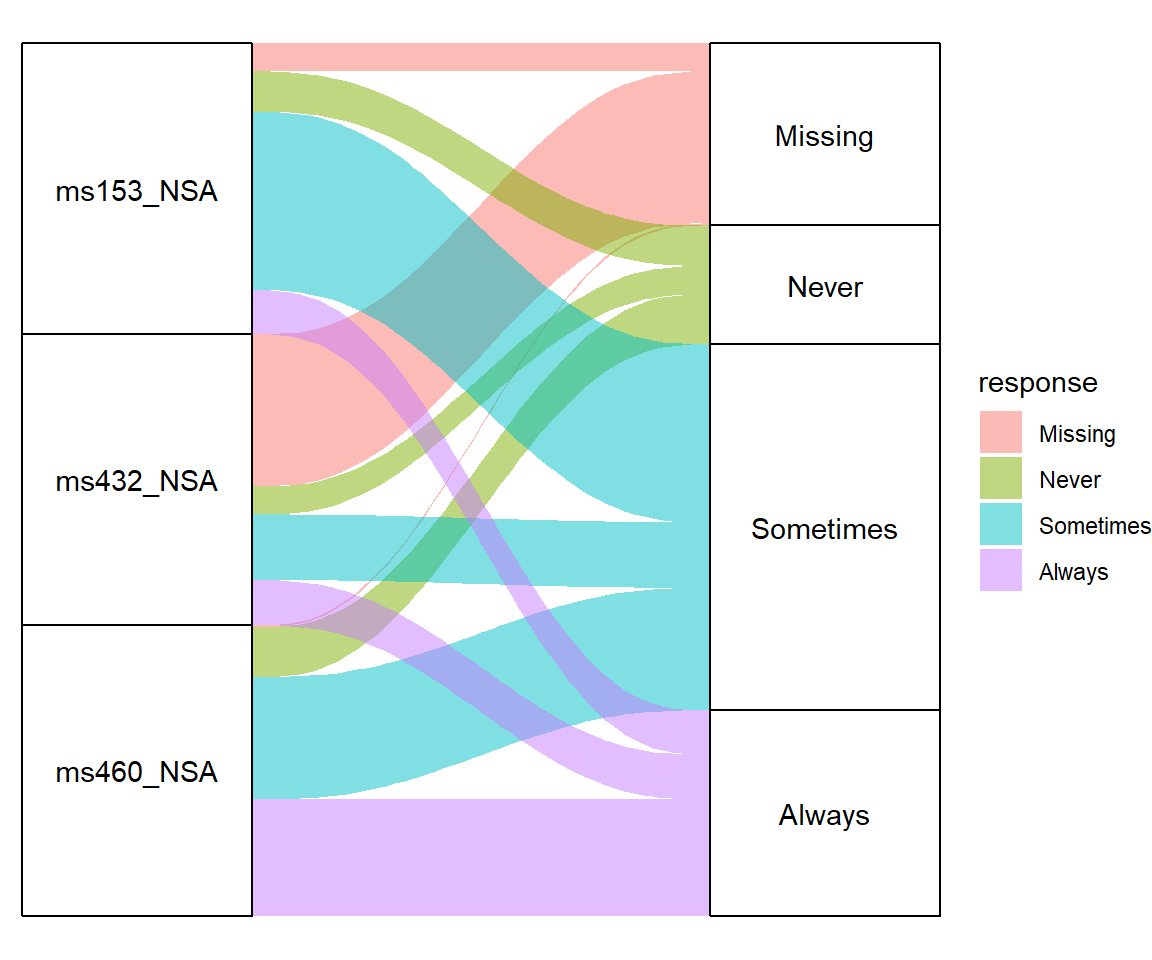
\includegraphics[width=10cm, height=7cm]{alluvial-plot-quintic.png}
    \centering
\end{figure}

\subsection*{Map}
\begin{figure}[h]
    \centering
    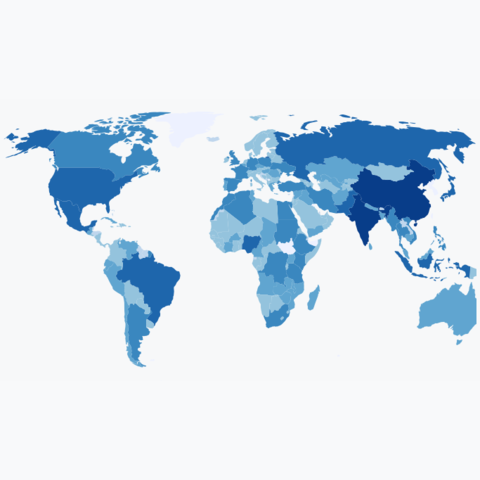
\includegraphics[width=10cm, height=7cm]{choropleth_basic.png}
    \centering
\end{figure}

\newpage

\subsection*{Line Chart}
\begin{figure}[h]
    \centering
    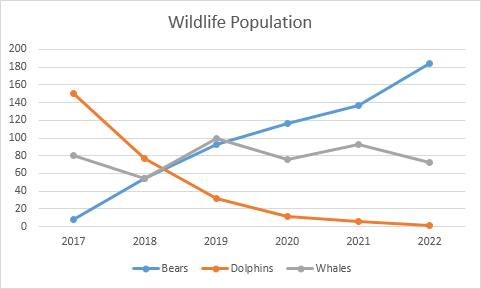
\includegraphics[width=10cm, height=7cm]{line-chart.png}
    \centering
\end{figure}

\end{document}